\chapter{The CMS experiment at the LHC}
\label{chap:xlhcms}
\minitoc
\myepigraph{[...]: l’esprit d’une nation réside toujours dans le petit
  nombre, qui fait travailler le grand, est nourri par lui, et le
  gouverne.}{Voltaire, in \textit{Essai sur les mœurs et l'esprit
  des nations}}


In this Chapter, I present the experimental setups
deployed at CERN to produce and record ultrarelativistic nuclear
collision data. The Chapter begins with a description of the
accelerator chain behind the Large Hadron Collider, before detailing the LHC itself,
emphasising on the various collision setups and energies achieved so
far. The discussion then moves to the experiments placed at the four
interaction points, with a natural focus on the one that produced the
data used in this Thesis, the Compact Muon Solenoid. The CMS detector
geometry and components are defined, with a focus on the parts which
are the most exploited here.



\section{The Large Hadron Collider}
The Large Hadron Collider~\cite{Evans:2008zzb} is the machine based at
CERN to study elementary particle physics of the Standard Model and beyond, by
the means of accelerating and colliding beams of atomic nuclei to the highest
energies ever made by men. The beams are injected into the LHC
after having followed several refinement steps in other particle accelerators
presented below. After injection into the LHC,
the beam energies are ramped up to the desired collision energy, in a
process detailed in Section~\ref{sec:lhcsetups}. The experiments are
provided with parts of the available beams that are squeezed in the
interaction points to provoke collisions. Detectors are placed at interaction points 1, 2,
5 and 8, and these would be presented in Section~\ref{sec:experiments}.
\subsection{Acceleration devices}
\label{sec:accdev}

The LHC is an accelerator and a collider maintained at CERN near
Geneva (Switzerland), inside the 27 kilometer tunnel previously hosting
the LEP machine. The tunnel has eight straight sections, eight
arcs, and eight underground access shafts. The LHC tunnel is connected
to the rest of the CERN accelerator complex by two transfer tunnels
(named TI2 and TI8, see Figure~\ref{fig:cern}) of $\sim$ 2.5 kilometer length.

A simplified picture of the LHC and its injector chain is presented in
Figure~\ref{fig:cern}. The linear accelerators (LINAC) are
present at the beginning of the injection chain: LINAC2 is used as a
proton accelerator, and LINAC3 serves as ion accelerator.

The LINAC2 provides low energy proton beams to the Proton
Synchrotron Booster (PSB). The protons arrive from LINAC2 at 50
MeV into the PSB, which further accelerates them to 1.4 GeV and
aggregates the beam in a bunch before delivering it to the
Proton Synchrotron (PS). The PS has various bunch filling schemes
possible for protons (8, 16 or 64 bunches per injection).
Protons are taken to an energy of 25 GeV prior to the ejection towards the
Super Proton Synchrotron (SPS), in bunches of 10$^{11}$ protons
each. The SPS further accelerates the proton beam to 450 GeV and can
store up to 240 bunches per fill~\cite{Schindl:384396}. 

\begin{figure}[h]
  \begin{center}
    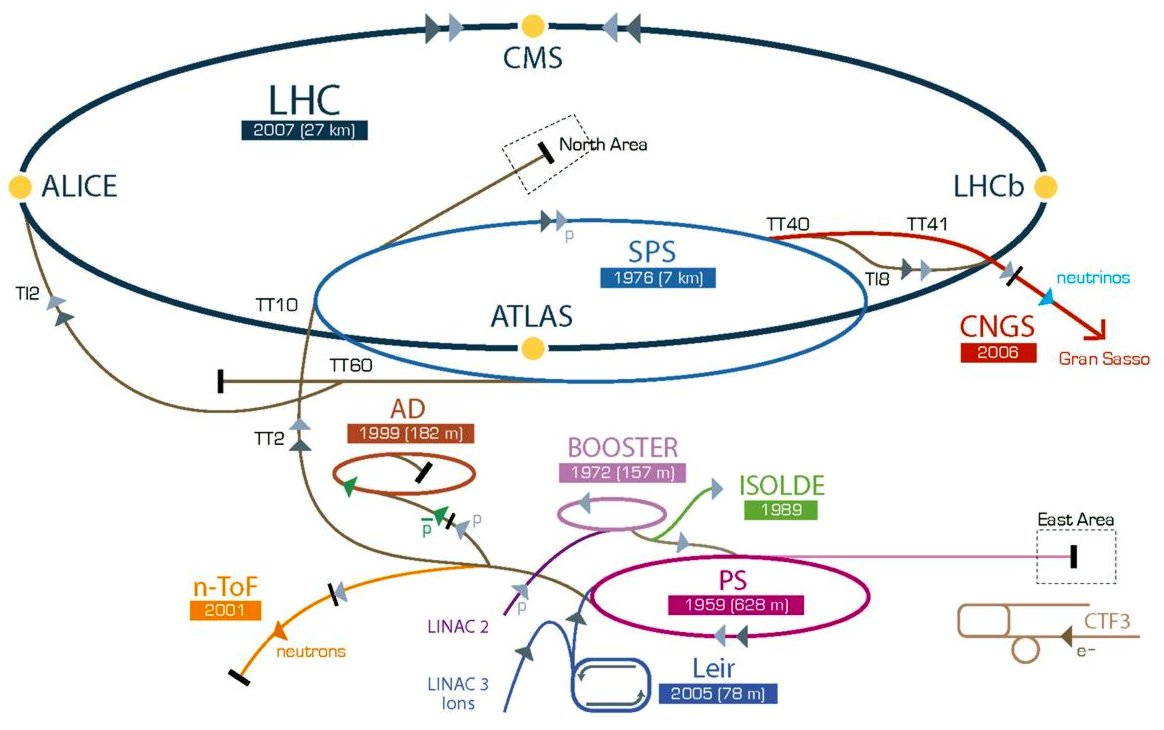
\includegraphics[width=0.8\textwidth]{Chapters/xLHCMS/cernschema.jpg}
    \caption{The CERN injection and acceleration chain for LHC
      experiments. Relative positions and sizes are not to scale.}
    \label{fig:cern}
  \end{center}
\end{figure}

Lead ions do not follow the same route as protons. Ions are generated
in LINAC3, which communicates its pulses to the Low
Energy Ion Ring (LEIR). The LEIR accumulates up to 4 bunches of
Pb$^{54+}$ beams at 0.0148 GeV per unit charge (GeV/$u$), which are
then sent to the PS. During the PS
acceleration up to the SPS injection, the remaining charges are stripped from the ion
beams, and the required LHC bunch spacing (125 ns) is attained. The
energy per unit charge is also increased from 4.26 GeV/$u$ to 177
GeV/$u$, and the number of bunches in the SPS train increases from 4
to 52~\cite{Schindl:384396}.



The proton or ion beams are carried into the LHC tunnel from two
injection tunnels going in opposite directions. The injected beams are
then cycling in the tunnel until the energy and current requirements
are met.


\textbf{Acceleration} of the LHC beams is performed with superconducting
radiofrequency cavities, that are set to work in the proton
acceleration case at a 400 MHz frequency (i.e. 25 ns spacing between
$p$ bunches) and operating at 4.5 K~\cite{Arnaudon:2004kq}.

In the case of Pb ions, the settings are slightly different: inevitable limitations to the beam stability arise when accelerating Pb nuclei, such as
intra beam interactions (e.g. electron capture by pair production)~\cite{Beuret:2004mf}. All known limitations to the brightness
of ion beams were studied from previous experience at other facilities
such as PETRA or HERA, and led to reduction of the luminosity of beams
injected in the LHC to prevent heat-induced magnet quenches~\cite{jowett}.


\textbf{Bending} of the LHC beams is achieved by the magnet
system. The arc sections of the LHC comprise 7000
multipole magnets, the most important of them being the 1232
dipoles, weighing about 35 tons. Quadrupoles and higher order multipole magnets are also used
to maintain the transverse shape of the beam.% during the bending
%process.


The dipole magnets are made of niobium-titanium (Nb-Ti)
superconductive coils powered at up to 12 kA and maintained in their
superconductive state by a single 1.9~K helium fueled cryostat. In
achieving a 7~TeV beam energy (i.e. in $pp$ collisions at \s~=14 \TeV),
the magnets would produce a 8.33 Tesla field strength.




% When propagating in the beam pipes, the beams have a spatial
% extension, a transverse and a longitudinal motion, that ought to be
% monitored at any point. These accelerator parameters can be used ot
% derive the beam luminosity.


% Especially, all beam-beam interactions that
% are considered in the design of the magnet sections and straight
% sections
% resulting in a loss of nuclei also results in a heat load that must be
% contained below the quench limit of superconducting magnets.

\subsection{LHC setups and energies}
\label{sec:lhcsetups}


From the Run1 startup in 2008 to the beginning of the Run2 proton-proton
data taking in 2015, the LHC has delivered experiments with an ever
increasing energy and luminosity, in $p$ or Pb
beams. Table~\ref{tab:collisions} sums up the energy and luminosity
delivered to the CMS experiment from the 2010 start\footnote{On
  September 19, 2008, an electrical fault occurred in a ramp up test
  in Sector 3-4. The fault affected several dipoles and quadrupoles,
  releasing a two-ton 
  helium leak in the tunnel and delaying the LHC commissioning phase for
  approximately a year and a half.} to October 2015.
\begin{table}[h]
  \begin{center}
    \begin{tabular}{c|cccc||c}
      
      & 2010 & 2011 & 2012 & 2013 & 2015 \\
      \hline
      \multirow{4}{*}{ $pp$ }&\multicolumn{1}{c|}{\s~= 2.76~\TeV}&&&\multicolumn{1}{|c||}{\s~= 2.76~\TeV}&\\ 
      & \multicolumn{1}{c|}{\lumi~= 235~\invnb}  & & &\multicolumn{1}{|c||}{\lumi~= 5.6~\invpb}  & \\
      \cline{2-6}
      &  \multicolumn{2}{c|}{\s~= 7~\TeV}& \multicolumn{1}{c}{\s~= 8~\TeV} &\multicolumn{1}{|c||}{}&\s~=13~\TeV \\ 
      & \lumi~= 45~\invpb & \multicolumn{1}{c|}{\lumi~= 6.1~\invfb} &
      \multicolumn{1}{c}{\lumi~= 23.3~\invfb}
      &\multicolumn{1}{|c||}{}&\lumi~= 2.8~\invfb \\ 
      \hline
      \multirow{2}{*}{ $p$Pb }& & & &\multicolumn{1}{|c||}{\snn~= 5~\TeV}& \\ 
       & & & &\multicolumn{1}{|c||}{\lumi~= 36~\invnb}&  \\ 
      \hline
       \multirow{2}{*}{ PbPb }&\multicolumn{2}{c|}{\snn~= 2.76~\TeV}  & & & \\ 
       & \lumi~=9.3~\invmub  &\multicolumn{1}{c|}{\lumi~=184~\invmub}  & & & \\ 
      \hline
    \end{tabular}
  \end{center}
  \caption{LHC collision setup and energies from startup to October
    2015. Integrated luminosities correspond to what was \textbf{delivered} to
    CMS until Oct. 25$^{\rm th}$, 2015~\cite{lumi}.}
\label{tab:collisions}
\end{table}



\subsection{The LHC experiments}
\label{sec:experiments}
As we can see in Figure~\ref{fig:cern}, there are four main experiments on
the LHC path. These are situated at Interaction Points (IP) where
beam crossing occurs. Each experiment has its own collaboration of
institutes, researchers, and distinct physics programme:

\begin{itemize}
\item[] IP1 is where the \textbf{ATLAS} detector is placed. The ATLAS acronym
  stands for A Toroidal LHC Apparatus~\cite{Aad:2008zzm}. As its name
  suggests, the detector holds a toroidal magnet, supplementing a 2 T solenoid
  surrounding the tracker. The main goal of ATLAS is to study the
  Higgs mechanism and to search for physics beyond the Standard Model,
  although the collaboration also works on heavy ion
  physics~\cite{atlasHI}.
\item[] The \textbf{ALICE} (A Large Ion Collider Experiment) detector
  is located at IP2~\cite{Aamodt:2008zz}. It is a general purpose
  detector aiming at a precise study of QCD in extreme conditions,
  especially via its extended heavy ion physics programme. Its excellent
  particle identification capabilities permit a fine measurement of multiplicity, energy flow and heavy flavour measurements in ultrarelativistic heavy ion
  collisions~\cite{ALICE}.
\item[] The Compact Muon Solenoid \textbf{CMS} is located at IP5. CMS
  is a multipurpose detector, aiming first at the precise measurement
  of Higgs boson properties and couplings with other particles, as
  well as a search for physics beyond the Standard
  Model~\cite{Chatrchyan:2008aa}. The central feature of the CMS
  detector is a solenoid magnet of 3.8 T surrounding the trackers and
  calorimeters. Its muon chambers are especially precise at measuring
  muon hits up to the TeV scale with a momentum resolution below
  1\%. The CMS experiment also has a heavy ion programme (this Thesis
  is a part of it!), mostly steered towards a detailed study of parton
  energy loss and heavy flavour physics, but also capable of global
  heavy ion event measurements~\cite{CMSHI}. The CMS detector is
  discussed in more detail in the next Section.
\item[] At IP8, the LHC-beauty experiment (\textbf{LHCb}) is mostly
  dedicated to measuring rare physics processes involving $b$ quarks, $CP$ violation
  and the search for beyond-Standard-Model physics in the flavour
  sector~\cite{Alves:2008zz}. There are two specifities in the LHCb
  detector:
  First, the detector is fully instrumented in only one side of the
  interaction point with a dipole magnet around the outgoing (forward)
  beam direction. Second, the luminosity leveling ensuring a low
  (practically \textit{constant}) instantaneous luminosity from
  beginning to end of a data taking period. This is achieved by the
  LHC accelerator operators applying a slight transverse offset
  between the two beams. It also reduces the number of primary $pp$
  vertices (also known as pile-up), facilitating the tracking of
  particles, especially important in measuring the flight distances of
  heavy hadrons. Recently, the LHCb collaboration got more involved
  with a promising heavy ion physics programme~\cite{Jing:1757559}.
\end{itemize}


\section{CMS}
\label{sec:CMS}

The CMS detector will now be described. Although mainly conceived to
detect particles coming from $pp$ collisions, it can also perform well
in heavy ion collisions, as well as detecting cosmic ray muons. The
central feature is a superconducting solenoid magnet operating at 3.8
T, coupled with an iron yoke for magnetic flux return.
\subsection{General concepts}
\label{sec:general}

The CMS detector is placed in IP5 of LHC, in a cavern down an
approximately hundred meter deep shaft in Cessy, France. The detector weighs approximately 12.5
tons, is 15 meters in diameter and 21 meters long. Its precise
geographical location with respect to the rest of CERN sites can be
seen at the top of Figure~\ref{fig:topLHC}.

\begin{figure}[t]
  \begin{center}
    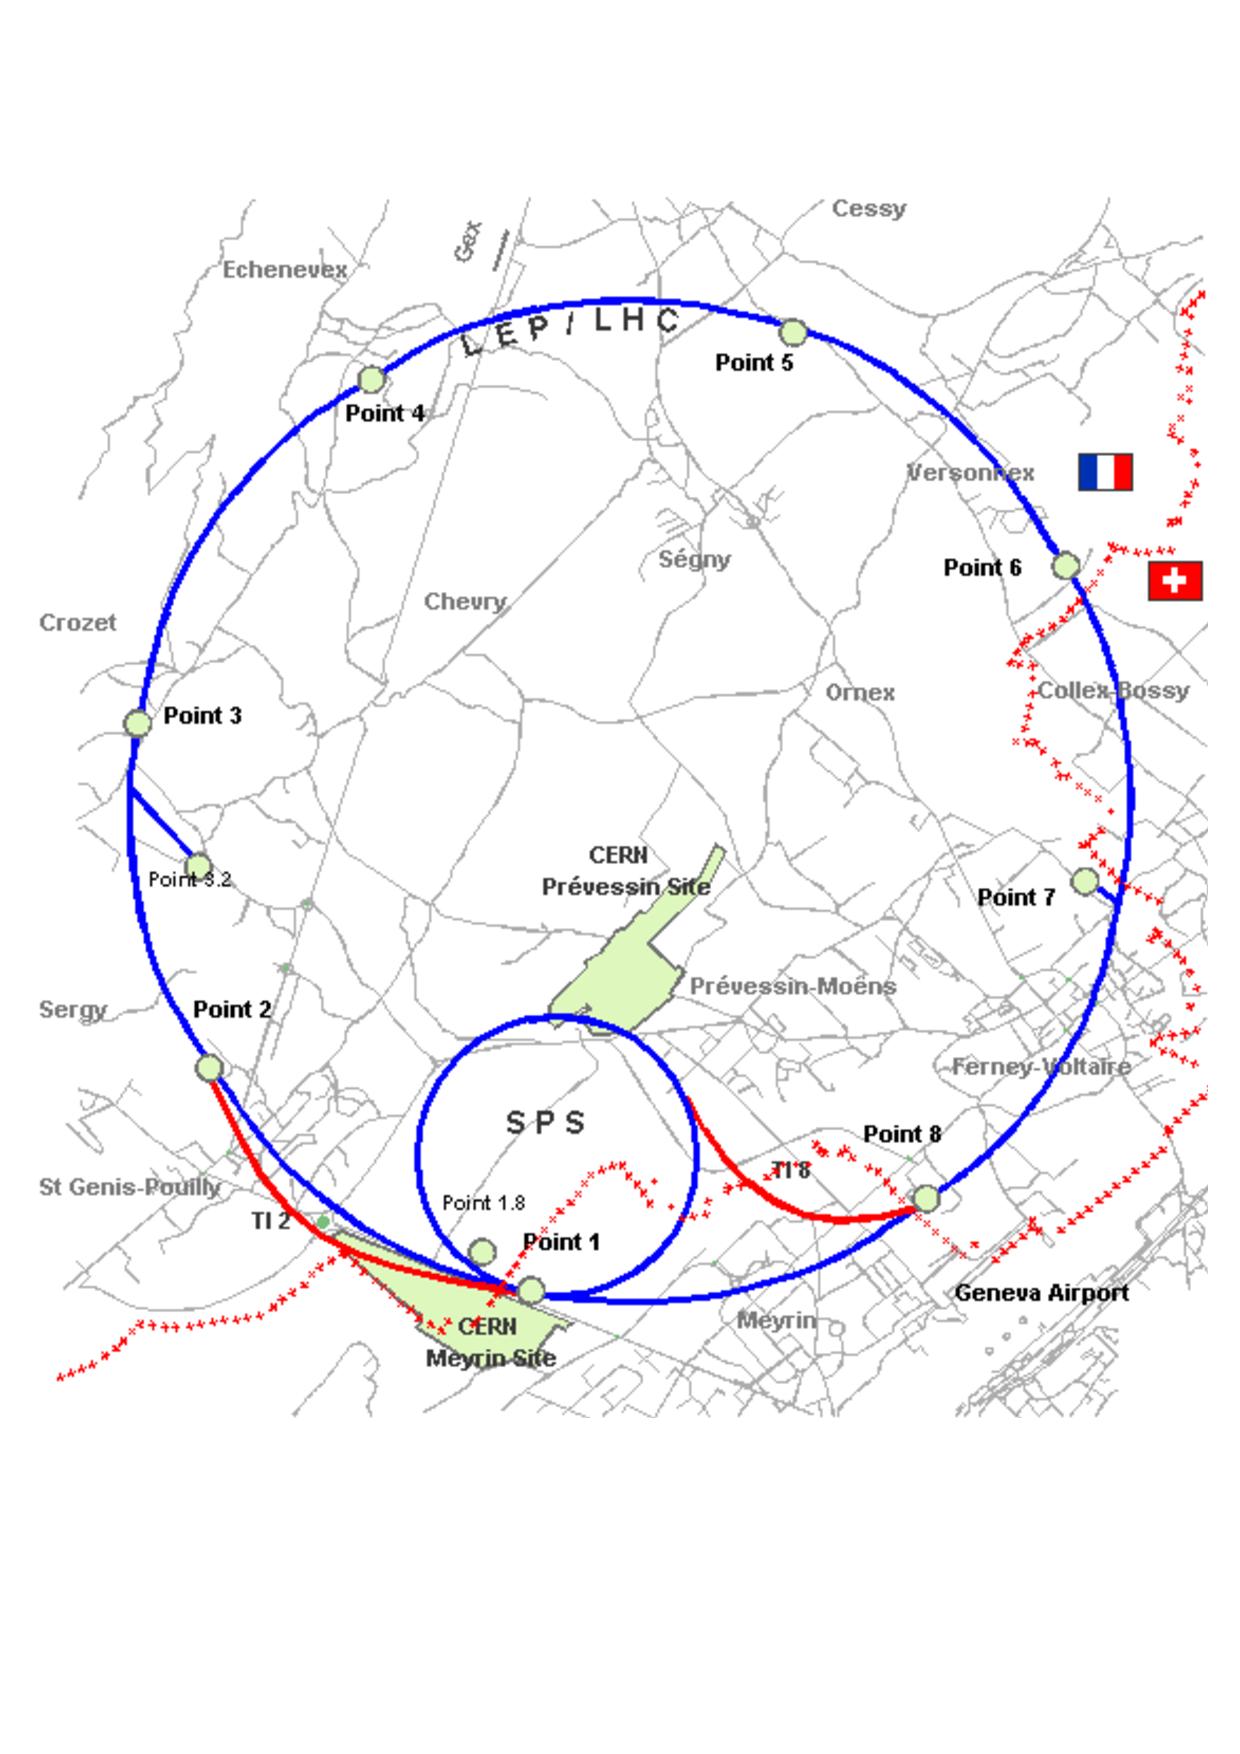
\includegraphics[width=0.8\textwidth]{Chapters/xLHCMS/maplhc.pdf}
    \caption{Top view of the SPS and LHC, including main CERN
      sites. CMS is located at Point 5.}
    \label{fig:topLHC}
  \end{center}
\end{figure}


 A schematic view of the CMS
detector is shown in Figure~\ref{fig:cutaway}.


The coordinate system used in CMS takes its origin in the nominal
collision point at the centre of the experiment, with the $y$-axis
pointing vertically upward, the $x$-axis pointing towards the center
of the LHC `circle', and the $z$-axis then pointing along one of the
beam directions, namely towards the Jura mountains (or in the
counterclockwise direction, when looking from above). The azimuthal
angle $\phi$ is measured in the $x-y$ plane with respect to the $x$ axis. The
radial coordinate $r$ is taken in the $x-y$ plane, and the polar angle
coordinate $\theta$ is measured from the
$z$-axis~\cite{Chatrchyan:2008aa}.

\begin{figure}[htb]
  \begin{center}
    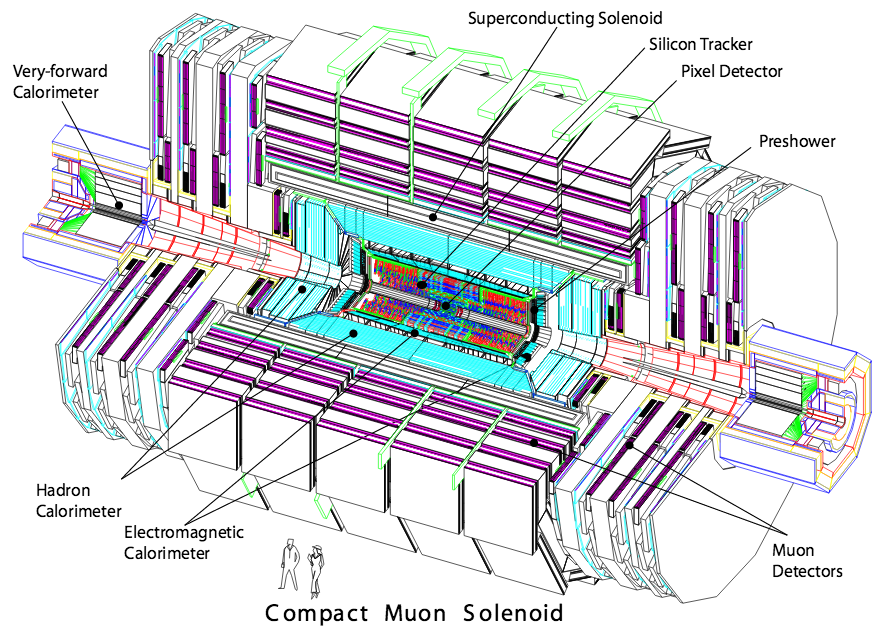
\includegraphics[width=0.8\textwidth]{Chapters/xLHCMS/cutawayCMS.png}
    \caption{Cut-away view of the CMS detector~\cite{Chatrchyan:2008aa}.}
    \label{fig:cutaway}
  \end{center}
\end{figure}


Pseudorapidity, the preferred experimental measure for angular
position of detected particles, is defined in
Equation~\ref{eq:eta}. 

\begin{equation}
\label{eq:eta}
\eta = - \textrm{ln tan} \frac{\theta}{2}
\end{equation}

Transverse quantities such as \pt, $E_{T}$,
and $E^{\rm miss}_{T}$ are computed in the $x-y$ plane.


The logic behind the detector design is governed by the necessity of
measuring large momentum muons with great accuracy. A large bending
power is thus necessary, hence the large magnetic field. The magnet is
thirteen meters long, its inner diameter is six meters and surrounded
by a complex return yoke of more than 1.5 meter thickness of iron in total,
with muon stations hitherto embedded. 


From the interaction point out, the subdetectors are:

\begin{itemize}
\item[-] The tracker system, composed of 3 layers of silicon pixel
  detectors and 10 layers of silicon microstrips;
\item[-] The elctromagnetic calorimeter (ECal), composed of transparent,
  radiation hard lead tungstate (PbWO$_{4}$) crystals;
\item[-] The hadron calorimeters (HCal), covering the barrel, endcaps
  and forward regions, and made of a brass/scintillator array of steel
  and light collection devices;
\item[-] Finally, the muon detector is a combination of drift tubes (DT) in
  the barrel and cathode strip chambers (CSC) in the endcaps,
  complemented by resistive plate chambers (RPC) in both regions.
\end{itemize}


\subsection{Trackers}
\label{sec:TRK}
To achieve most of its physics programme, CMS needs fast and efficient track
and vertex reconstruction. The tracking system evolves in high
multiplicity environments, either due to the multiple $pp$
interactions piling up in a single bunch crossing or due to a single heavy
ion collision. The trackers are contained in a cylindrical volume of
5.8 meters in length and 2.5 meters in diameter.

% \begin{itemize}
% \item[-] TOB
% \item[-] TIB
% \item[-] TEC
% \end{itemize}



To cope with the track multiplicity, the number of primary and
secondary vertices, a high granularity and quickly responsive system
is needed. Although this is achievable by repeating the layers of
sensitive material, there is a compromise to be found with the amount
of material, to minimise multiple scattering, and the cooling of
electronics when the tracker operates, as the whole tracker is plunged
in the solenoid magnetic field. 


The CMS tracking system is split in two main parts: the silicon pixel
detectors and the silicon strip tracker. The closest subdetector to
the interaction point is the pixel detector, as can be seen to the center of Figure~\ref{fig:tracker}.

\begin{figure}[htb]
  \begin{center}
    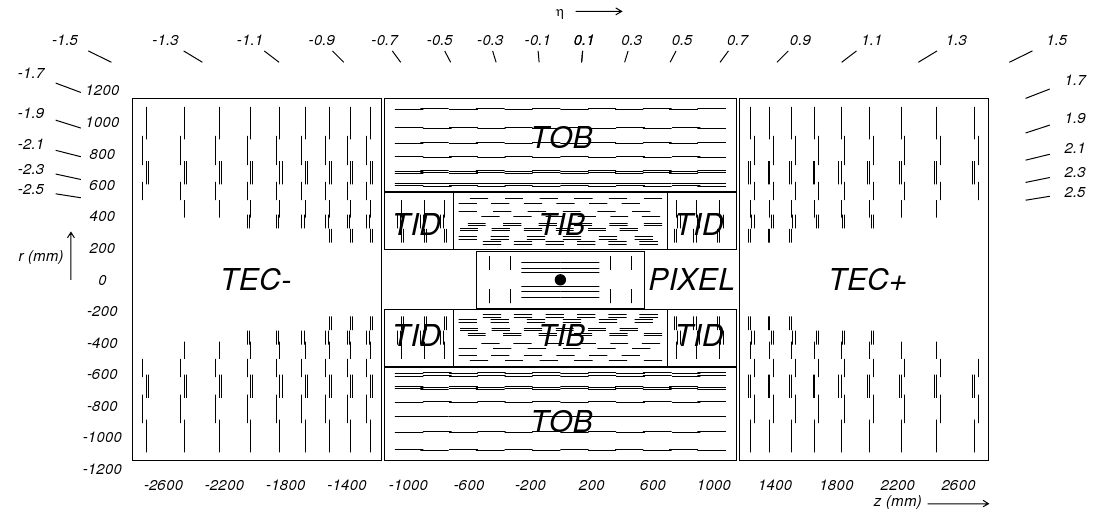
\includegraphics[width=0.8\textwidth]{Chapters/xLHCMS/fig_cmstracker.png}
    \caption{Schematic view of the sensitive areas in the CMS tracker system.}
    \label{fig:tracker}
  \end{center}
\end{figure}


The Pixel detector comes in 3 layers in the barrel and 2 disks at each
endcap. The barrel layers are concentric, within 4.4 to 10.2
centimeters of radius.

The strip tracker has 10 detection layers in the barrel extending
outwards, up to 1.1 meter of radius (forming the TIB and TOB subdetectors). Each endcap contains 9 disks of
silicon strips (forming the TEC subdetector), and the full system covers the pseudorapidity range
$\vert\eta\vert < 2.5$. 

The Pixel detector is made of 1440 pixel modules, and the strips
contain 15148 modules. In total, there is
about 200 square meters of sensitive silicon area in the tracker.


Using pixelated cells at radii below 10 cm is necessary for the occupancy
of the full system to be kept as low as possible, typically of the
order of 1\%. The pixel cells are 100$\times$150 square micrometers
wide, and the multiplication of layers allows a three dimensional
vertex reconstruction in space. In total, the barrel (BPix) and
endcaps (FPix) contain 48 million and 18 million pixels,
respectively. The 3.8 T field acts strongly on the
Lorentz drift (\textbf{E}$\times$\textbf{B}) of electron-hole pairs, resulting in charge sharing
between adjacent cells. Adjacent FPix modules are tilted of 20 degrees
in a turbine geometry to achieve a spatial resolution of 15 to 20
micrometers~\cite{Chatrchyan:2008aa}.



 When moving away from the interaction point, the
particle flux reduces, allowing the use of micro-strips of variable
sizes and pitches, depending on the position (inner or outer, barrel
or endcap). The four Tracker Inner Barrel (TIB) and the three Disk
(TID) layers (cf. Figure~\ref{fig:tracker}) are conceived in 320
micrometer thick silicon microstrip sensors of variable pitch,
achieving up to 4 $r-\phi$ measurements on a trajectory with a single
point resolution of about 30 micrometers. The outer barrel (TOB) and
endcap (TEC) layers provide another 6 and 9 $r-\phi$ measurements,
respectively, with respective single point resolutions of 35 to 50
micrometers. Figure~\ref{fig:trkperf} shows some of the performance of
the tracker system on muons in a $pp$ collision environment. On the left panel, the resolution of
transverse momentum for muons of 1, 10 and 100 \GeVc~is displayed
\vs. pseudorapidity. On the right hand side, the track reconstruction
efficiency for muons, of 99\% percent in most regions, is displayed
for the three \pt~regimes.


\begin{figure}[htb]
  \begin{center}
    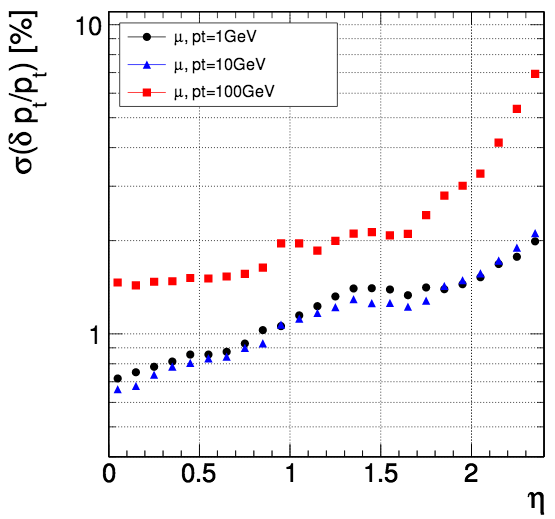
\includegraphics[width=0.45\textwidth]{Chapters/xLHCMS/trackermuonpt.png}
    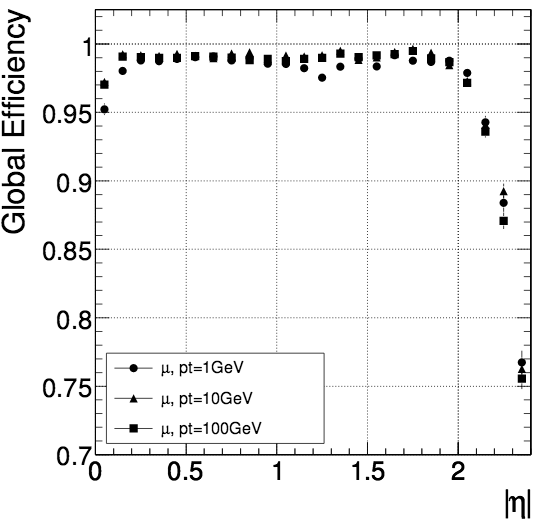
\includegraphics[width=0.45\textwidth]{Chapters/xLHCMS/trackermuoneff.png}
    \caption{\pt~resolution (left) and efficiency (right) for single muons
      reconstructed with the tracker system of CMS~\cite{Chatrchyan:2008aa}.}
    \label{fig:trkperf}
  \end{center}
\end{figure}



\subsection{Electromagnetic calorimetry}
\label{sec:ECAL}
The electromagnetic calorimeter (ECal) is made of 61200 lead tungstate
(PbWO$_4$) crystals mounted side by side in the barrel, plus 7324
adjacent crystals in each endcap, forming a hermetic and homogeneous
detector. One of the prime goals of this detector is the precise
detection of Higgs bosons decaying to two photons, maintaining a high
energy resolution and fine granularity.

The ECal is placed between the trackers and hadron calorimeters of
CMS. On Figure~\ref{fig:ecal} is shown an ECal crystal and the way they
are arranged. The granularity is 360-fold in the $\phi$ coordinate and
170-fold in $\vert\eta\vert$, amounting to a total of 61200
crystals. The light collection occurs at the far end of each crystal,
using avalanche photodiodes (APD) in the barrel and vacuum
phototriodes (VPT) in the endcaps. One endcap crystal apppended with
its VPT is displayed on the left of~\ref{fig:ecal}. The scintillation
properties of the crystal are expected to decrease with radiation
damage over the years of CMS operation, and a dedicated laser
injection system was put in place to track and correct the crystals ageing.

\begin{figure}[htb]
  \begin{center}
    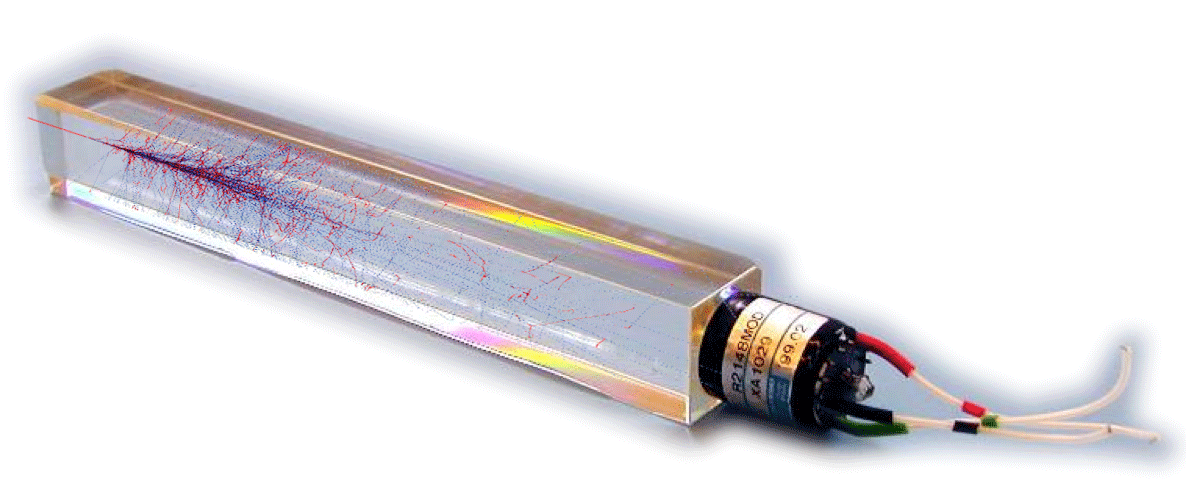
\includegraphics[width=0.3\textwidth]{Chapters/xLHCMS/CrystalWithVPTwithShower.png}
    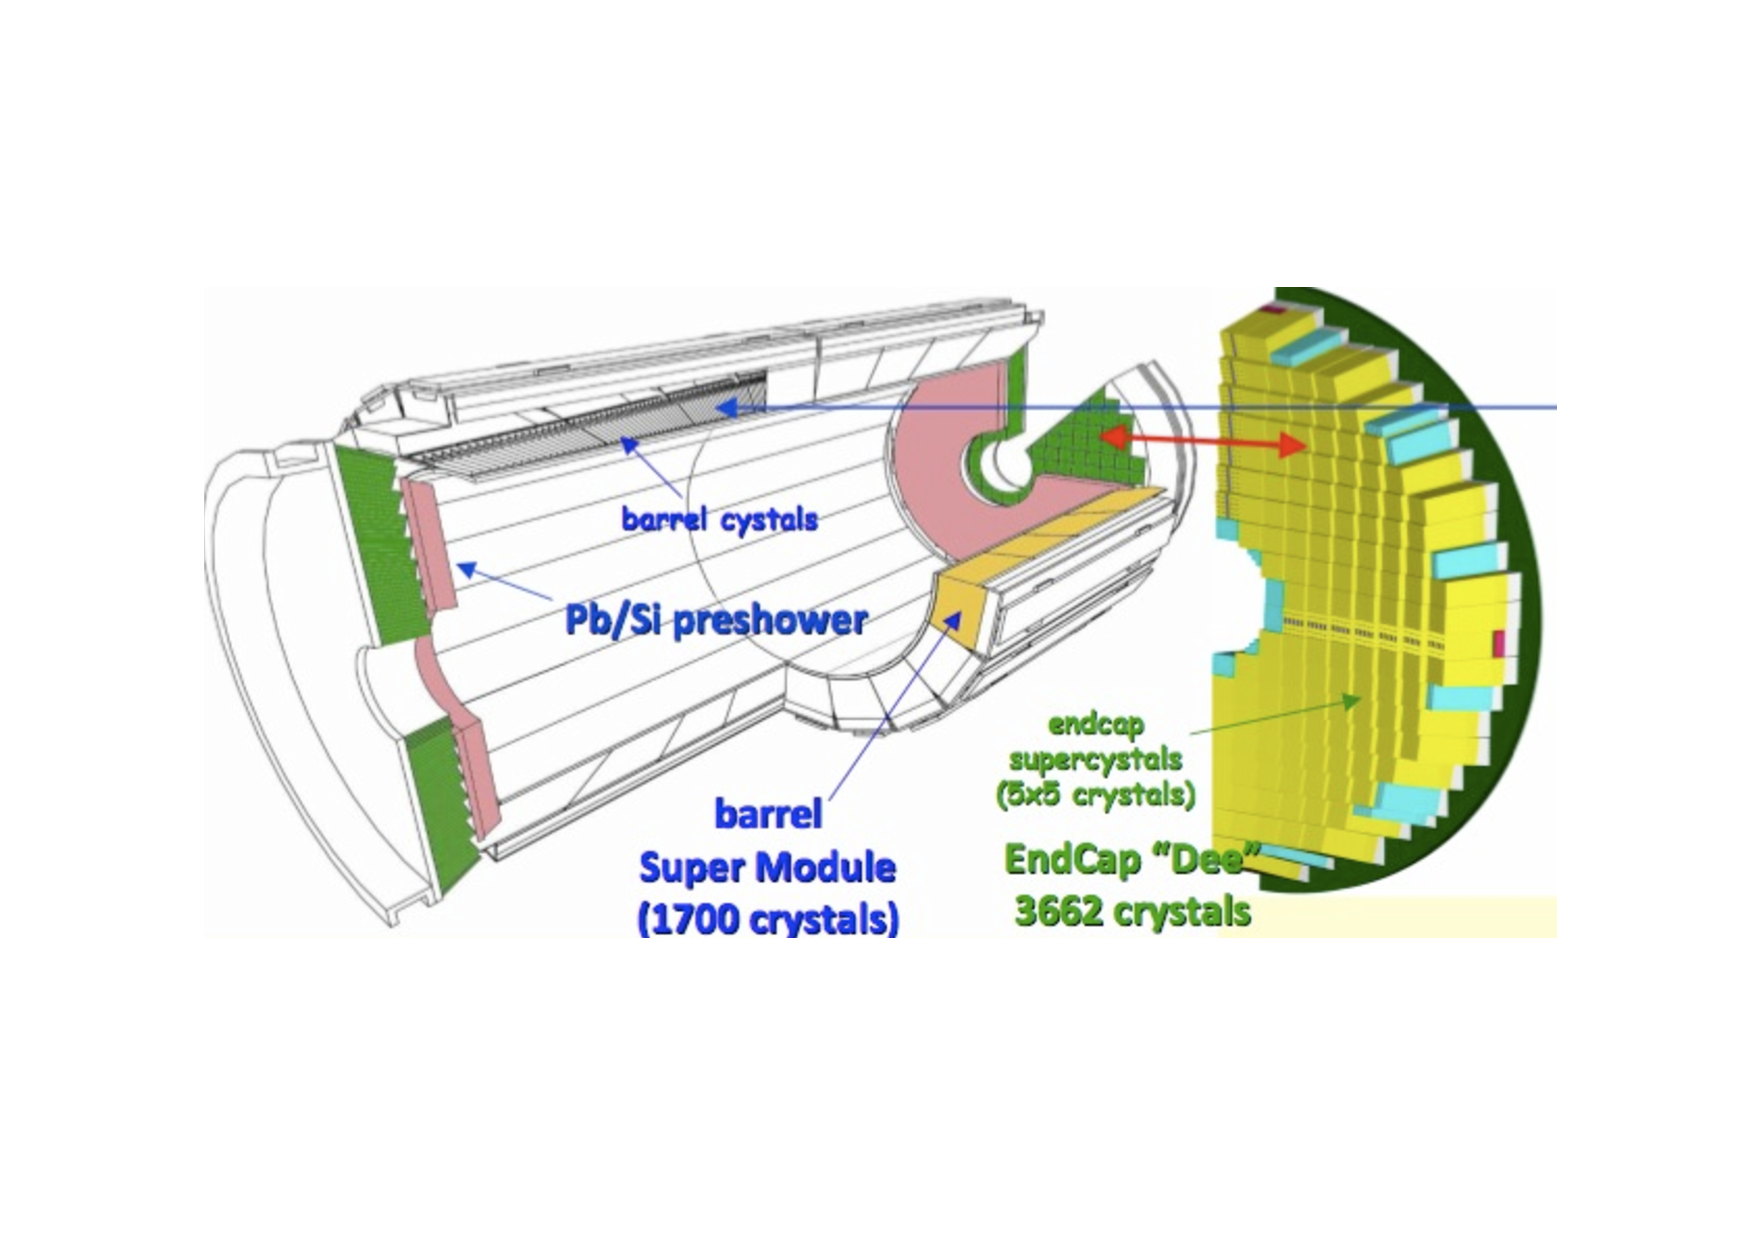
\includegraphics[width=0.6\textwidth]{Chapters/xLHCMS/ecal.pdf}
    \caption{Features of the electromagnetic calorimeter of CMS. Left: artistic view of a particle shower in a forward ECal
      crystal, with VPT collector downstream. Right: cut-away overview of the
      full ECal.}
    \label{fig:ecal}
  \end{center}
\end{figure}

The PbWO$_4$ crystals have a density of 8.28 g/cm$^{3}$, a high
refractive index of $n$ = 2.29 at peak wavelength and emit blue-green
scintillation light (420-430 nanometers). At room temperature, the
light output is low: 4.5 photoelectrons per MeV, uniformly over the 23
centimeter length of the crystal.

    
The ECal energy resolution is computed as a function of electron
energy as the sum of a stochastic term (S), a noise term (N) and a
constant term (C), as defined in Equation~\ref{eq:ecalres}. The
resulting energy resolution is shown in Figure~\ref{fig:ecalres}.

\begin{equation}
\left(\frac{\sigma(E)}{E}\right)^{2} =
\left(\frac{S}{\sqrt{E}}\right)^{2} + \left(\frac{N}{E}\right)^{2} +
C^{2}
\label{eq:ecalres}
\end{equation}

\begin{figure}[htb]
  \begin{center}
    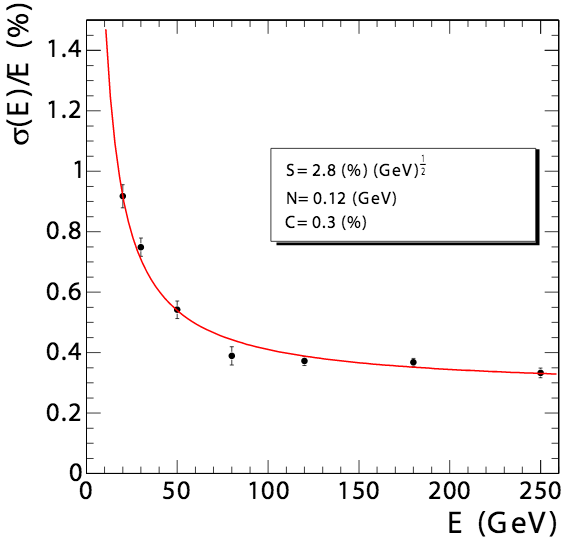
\includegraphics[width=0.6\textwidth]{Chapters/xLHCMS/resolutionECAL.png}
    \caption{ECal energy resolution as a function of electron energy~\cite{Chatrchyan:2008aa}.}
    \label{fig:ecalres}
  \end{center}
\end{figure}

\subsection{Hadronic calorimetry}
\label{sec:HCAL}
Hadron calorimetry plays an important role in the measurement of jets, total
energy deposits, or in the detection of specific topologies as two
forward energy jets with a large empty region between the two
(known as a \textit{rapidity gap}). The HCal of CMS is contained
between the ECal and the magnet coil, as is shown in
Figure~\ref{fig:HCal}.

\begin{figure}[htb]
  \begin{center}
    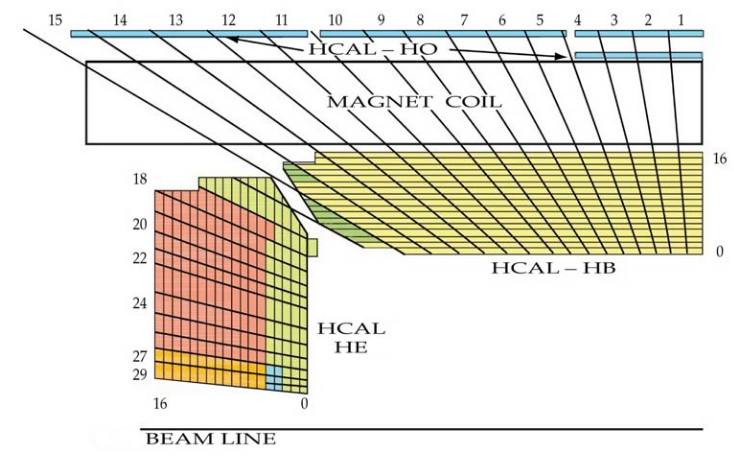
\includegraphics[width=0.6\textwidth]{Chapters/xLHCMS/HCAL.png}
    \caption{Hadron Calorimeter of CMS (HCal).}
    \label{fig:HCal}
  \end{center}
\end{figure}

The barrel section of the HCal (HB) is covering the pseudorapidity
range $\vert\eta\vert < 1.3$. It consists of 36 azimuthal wedges of
absorber forming two half barrels (HB+ and HB-) inserted from each side of the
magnet, combined with a plastic scintillator divided in 16 $\eta$
regions. Each wedge is composed of an innermost stainless steel plate,
a sampling of scintillating plastic tiles and flat absorber plates
made of brass (70\% Cu, 30\% Zn), a steel back-plate and a wavelength
shifting fibre exiting the wedge downstream of particle propagation.

Outside the vacuum tank of the solenoid stands the outer HCal (HO)
`tail-catcher', adding further sampling depth to the HB and
identifying late starting hadron showers.


The endcap HCal (HE) covers the range $1.3 < \vert\eta\vert < 3$, a
large region containing 13.2\% of the solid angle. The total 300 tons
of brass were produced from the decommissioning of over a million
World War II shell cases from the Russian navy, as is shown in
Figure~\ref{fig:urss}, completed with 1 million dollars worth of
American copper~\cite{URSS}.


\begin{figure}[htb]
  \begin{center}
    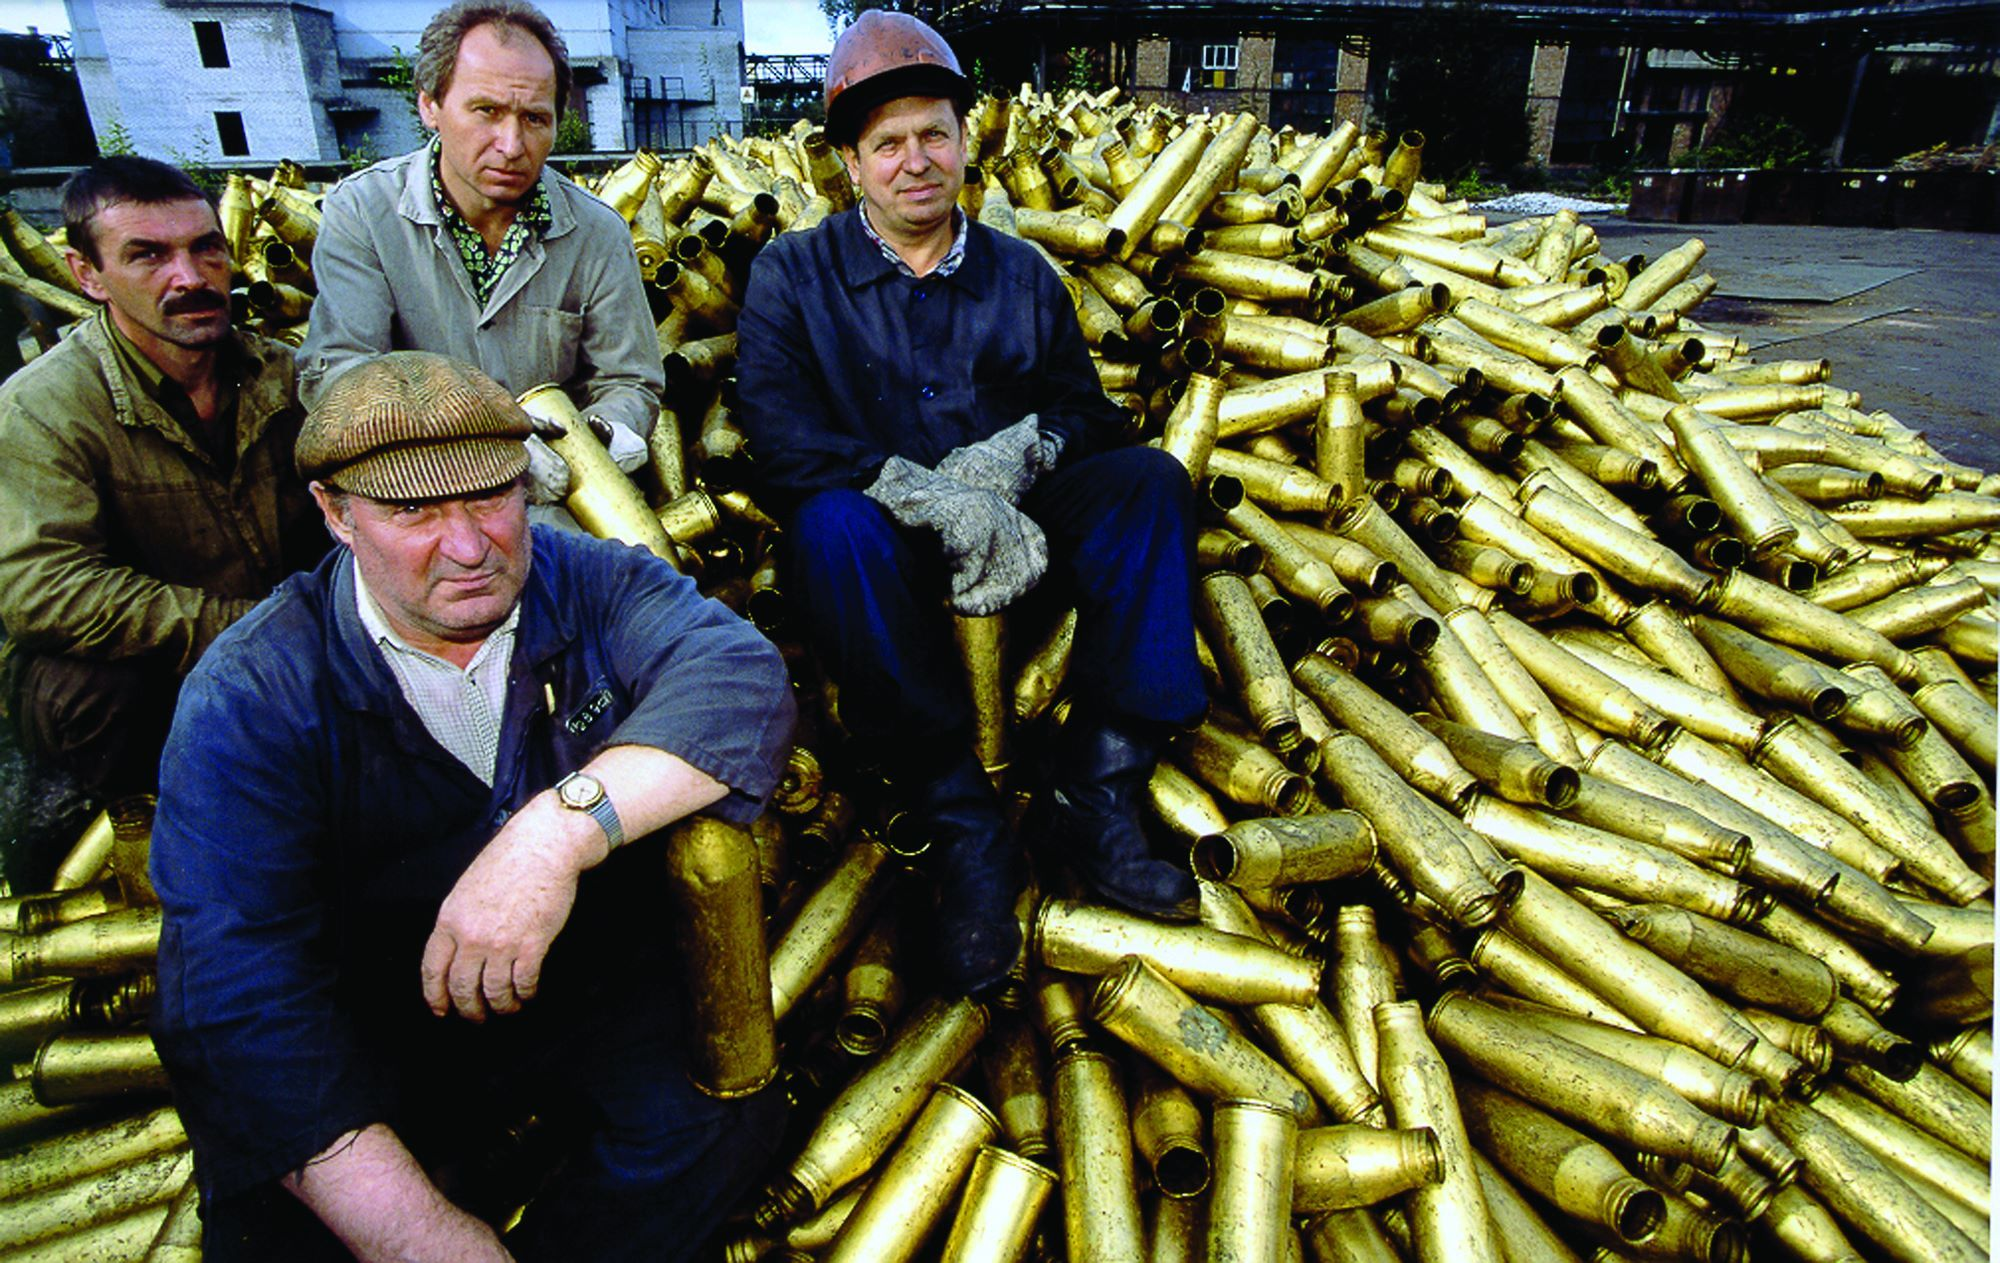
\includegraphics[width=0.6\textwidth]{Chapters/xLHCMS/urss.jpg}
    \caption{Russian navy shells re-used in the CMS Hadron Calorimeter.}
    \label{fig:urss}
  \end{center}
\end{figure}


The forward section of the HCal (HF) spans over 40\% of the available
phase space in CMS, in $3 < \vert\eta\vert < 5$. It was designed to sustain
unprecedented particle rate (10$^{11}$) and energy deposit (over 700
GeV in $pp$ collisions, and over 4 TeV in central PbPb
collisions~\cite{pbpbmult}). A schematic view of the HF is presented on
Figure~\ref{fig:HFpng}. The steel absorber is sampled with quartz
fibres that are insensitive to neutrons and produce Cherenkov light
guided towards the photomultipliers (PMTs), shielded behind 40
centimeters of steel, concrete and polyehtylene.


\begin{figure}[htb]
  \begin{center}
    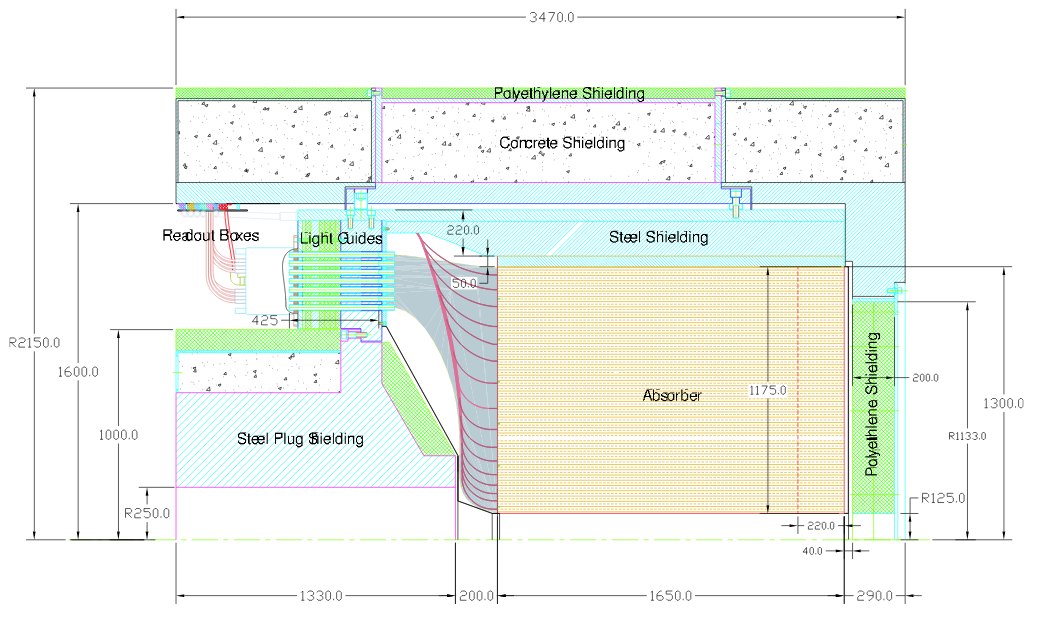
\includegraphics[width=0.7\textwidth]{Chapters/xLHCMS/HF.png}
    \caption{Cross section view of the HF calorimeter. The absorber is
    encased in steel and polyethylene shielding, and each tower is
    connected to light guides and PMTs situated 13 meters away from
    the beamspot (to the right)~\cite{Chatrchyan:2008aa}.}
    \label{fig:HFpng}
  \end{center}
\end{figure}

The HF can help tag forward jets, as well as measure a global event
activity, particularly useful in heavy ion collisions. The HF can be
used to infer the mean number of interactions per bunch crossing, the
luminosity in real time, and the centrality of a PbPb collision, as we
shall see in the next Chapter, Section~\ref{sec:centrality}.


Continuing to more forward directions, at $\vert\eta\vert < 8.3$ there
are the
Zero Degree Calorimeters (ZDC). Located at 140 meters on every side of
the CMS detector, these calorimeters are made of tungsten sampled with
quartz fibres, having the ability to measure neutral and charged particles
scattered at very small angles in diffractive $pp$ processes, as well
as to reconstruct the energy carried by spectator neutrons with a
resolution of 10\%.


\subsection{Muon chambers}
\label{sec:muonchambers}

The muon system in CMS is a crucial part of many
measurements. Particles are detected via a preferred signature often
including at least a muon, as in the case of quarkonium or heavy flavour
decays. In another energy range, the SM Higgs decaying to two Z
bosons would produce a 4 lepton decay, and the 4-$\mu$ channel was effectively detected with the CMS muon detectors. Even higher in
energy, the search for new heavy dimuon resonances may unveil
particles at the TeV scale, requiring an efficient and high-resolution
measurement at such muon momenta.

\begin{figure}[htb]
  \begin{center}
    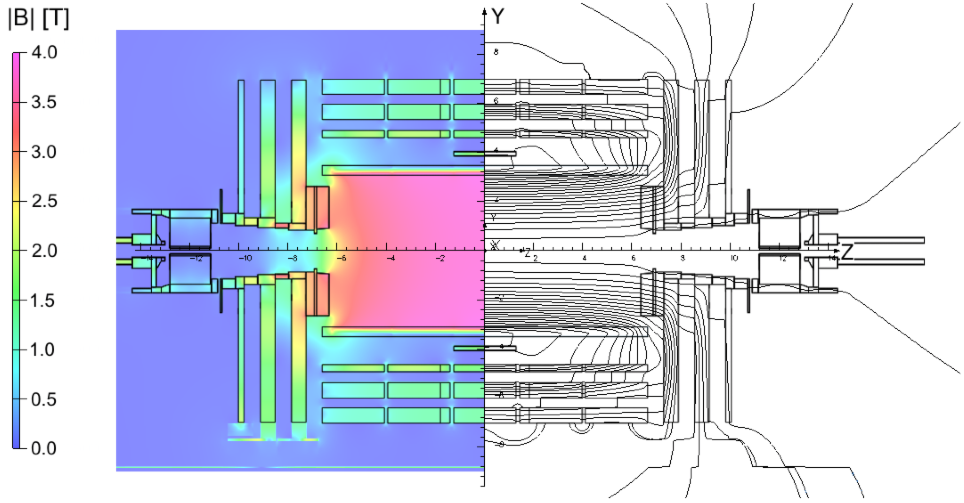
\includegraphics[width=0.7\textwidth]{Chapters/xLHCMS/MagField.png}
    \caption{Magnetic field intensity and field lines in
      CMS. Only insensitive material is displayed~\cite{Chatrchyan:2013sba}.}
    \label{fig:magfield}
  \end{center}
\end{figure}

As can be seen in Figure~\ref{fig:magfield}, the
magnetic field geometry is particularly complicated, with large \textbf{B}
gradients inside and around the return yoke (left part of the image:
field intensity), causing the field lines to curve back in the region
where muon stations are located. This delicate geometry over a wide
volume calls for a very high quality measurement of the position and orientation of outgoing muons, as well as a highly reliable alignment of
all subdetectors.


CMS uses three types of gaseous detectors to ensure muon triggering,
identification and reconstruction. With 25 000 square meters of
sensitive material, the muon chambers cover the barrel and endcap
region with up to 4 layers of muon stations embedded in the magnet's
iron return yoke. 
The muon stations are arranged in wheels around the solenoid and HCal endcap
regions, in the pseudorapidity range $\vert\eta\vert < 2.4$.

In the barrel region, the muon stations (in blue on
Figure~\ref{fig:muonstations}, left) combine Drift Tubes (DT)
stacked with Resistive Plate Chambers (RPC). In the endcaps, the RPC
are combined with Cathode Strip Chambers (CSC) (in pink on
Figure~\ref{fig:muonstations}, right).


\begin{figure}[htb]
  \begin{center}
    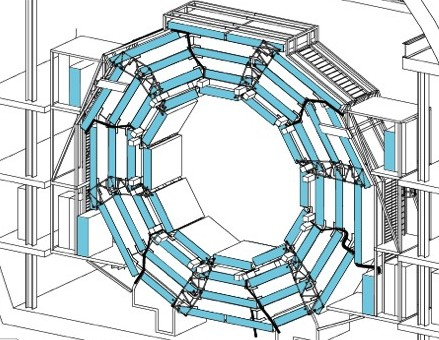
\includegraphics[width=0.55\textwidth]{Chapters/xLHCMS/dt-wheel.jpg}
    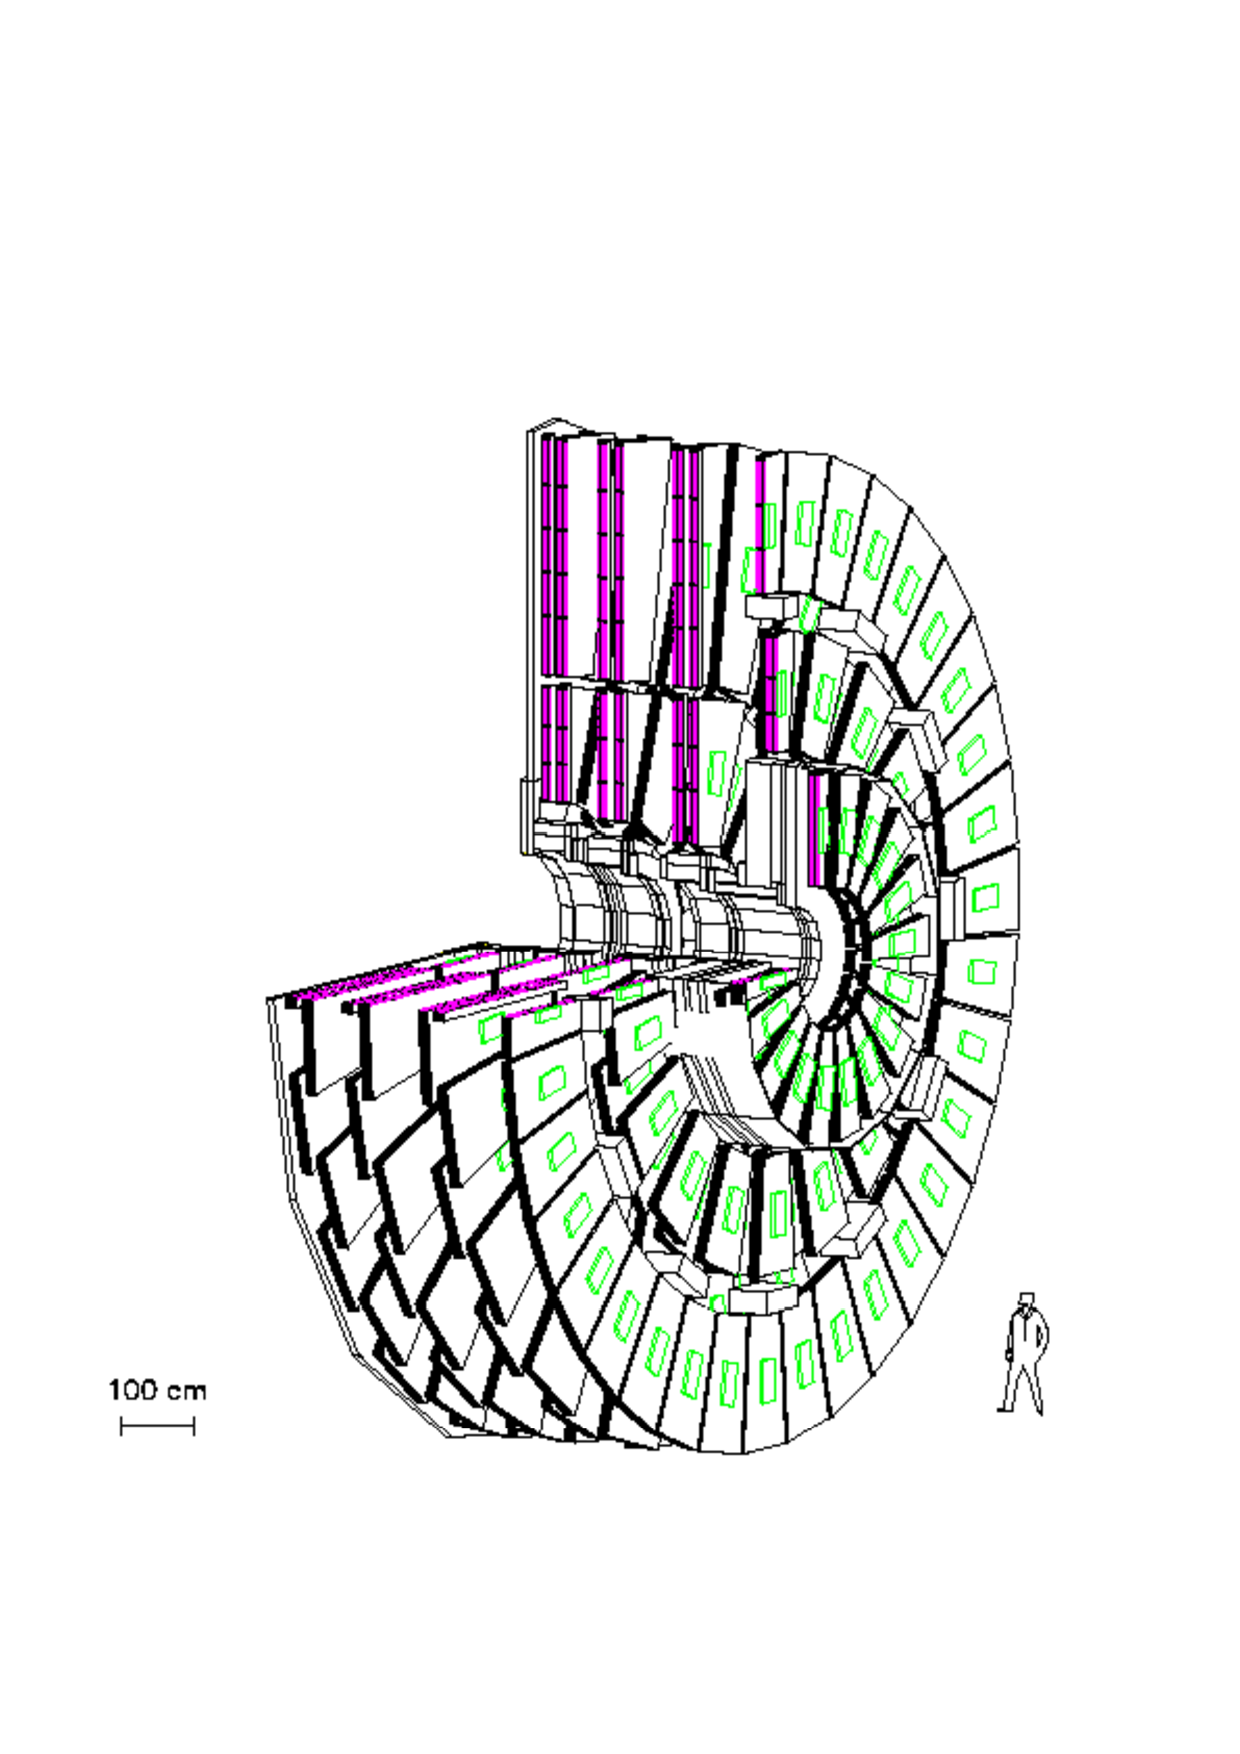
\includegraphics[width=0.42\textwidth]{Chapters/xLHCMS/csc-wheel.pdf}
    \caption{Barrel and endcap muon station wheels. Active material
     is displayed in colours. The reference axes belong to the right
     hand side figure~\cite{Chatrchyan:2013sba}.}
    \label{fig:muonstations}
  \end{center}
\end{figure}


The DTs cover the pseudorapidity range $\vert\eta\vert < 1.2$ in 4
cylindrical stations, embedded in wheels of the flux return
plates. The three innermost DT stations have 60 drift chambers and the
outer has 70. There are about 172 thousand sensitive wires of 2.4
meters each, over the full drift chambers. These are used as tracking
detectors for the barrel muon system.

%more detail on drift tubes

The interplay between RPC/DT, and CSC/DT subsystems can be clearly
seen in Figure~\ref{fig:muonsystem}.


\begin{figure}[htb]
  \begin{center}
    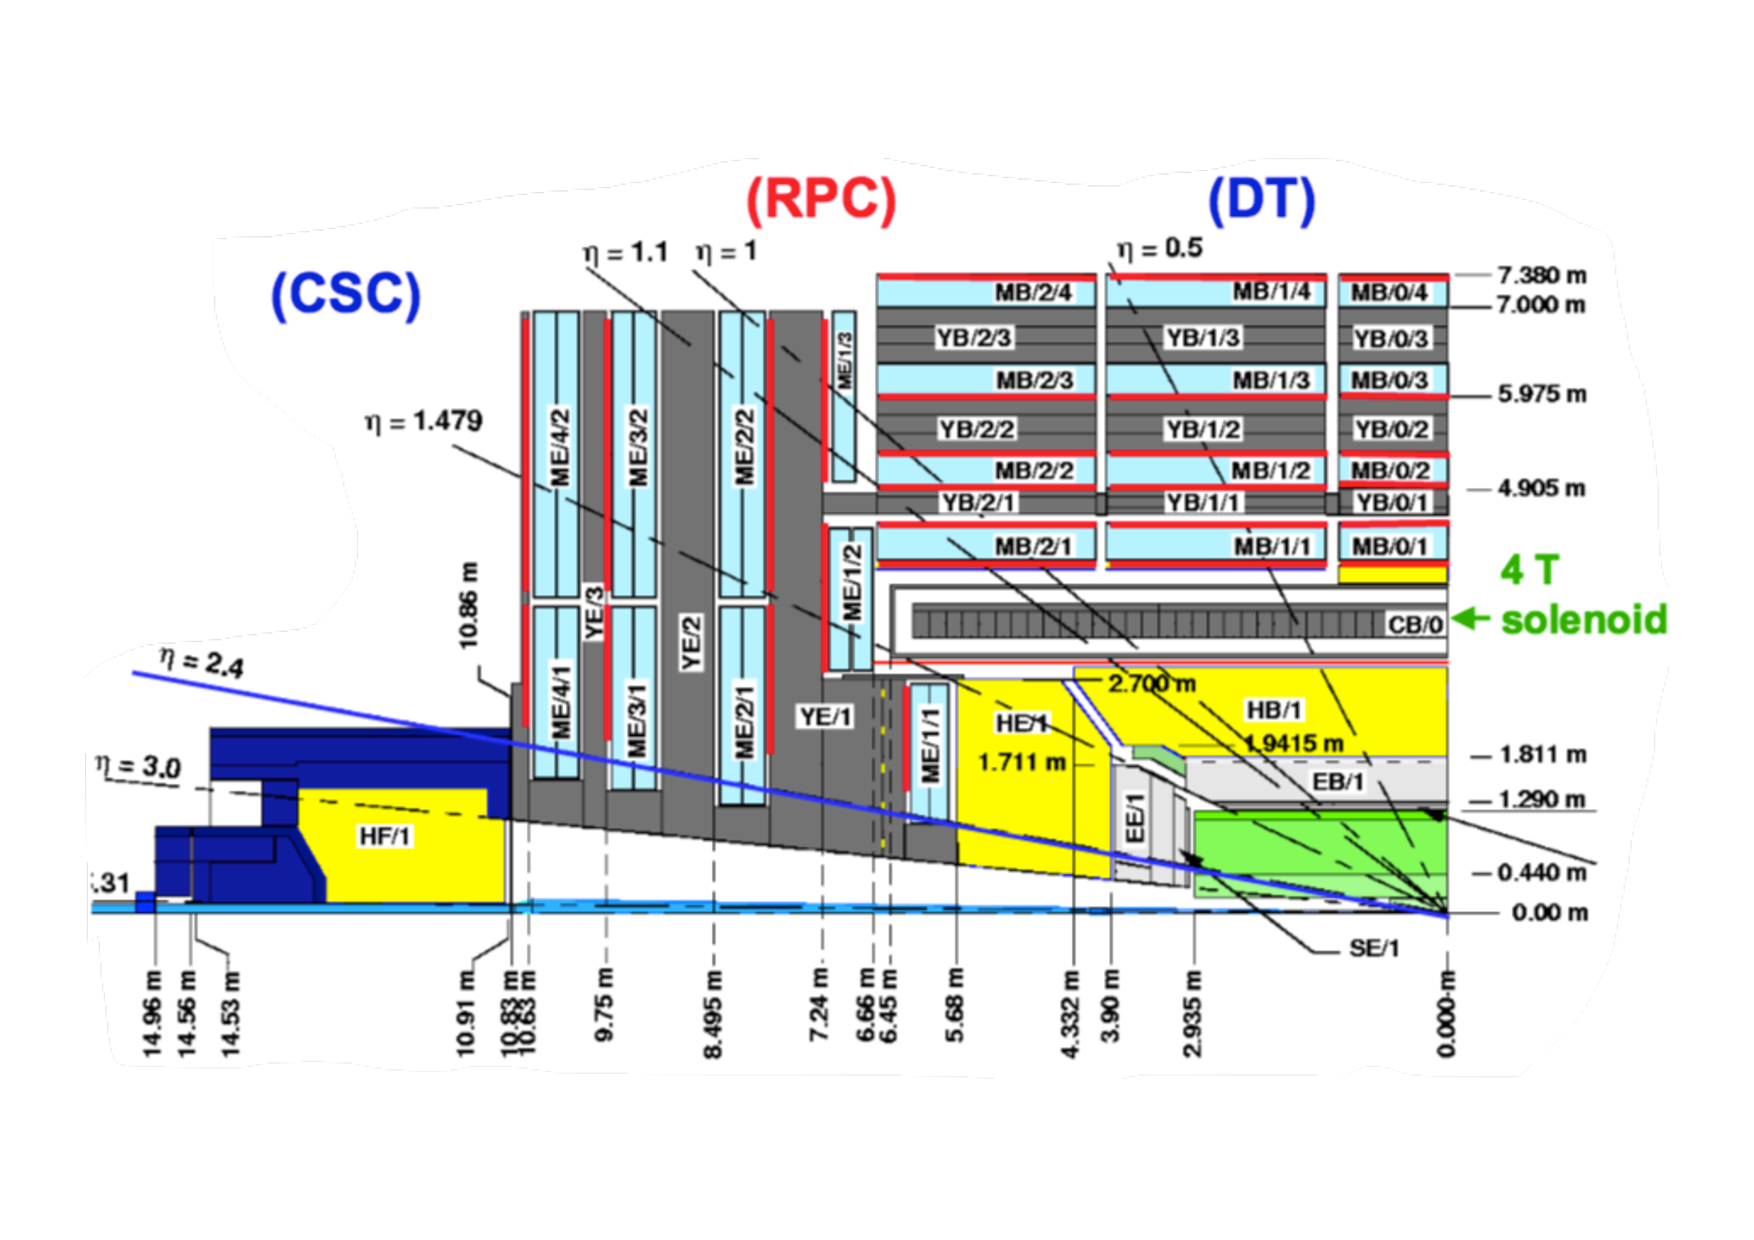
\includegraphics[width=0.78\textwidth]{Chapters/xLHCMS/muonsystem.pdf}
    \caption{Cross section view of the CMS detector, highlighting the
      muon detectors: RPCs are red, DT are in blue in the barrel
      wheels and CSC are blue in endcap wheels.}
    \label{fig:muonsystem}
  \end{center}
\end{figure}


A DT chamber comprises two or three independent blocks, called SuperLayers (SL), of
4 layers of rectangular drift cells, separated by a honeycomb
plate. The whole SL+honeycomb+SL system is inbetween RPC
plates. The full DT-RPC set are encased together in the iron yoke, but
act independently. The inner SL measures the $\phi$ position where a
muon entered the chamber. The muon then passes through the honeycomb,
reaches a second SL measuring $z$  (always
present in the 3 innermost stations, never in the fourth station). The
third SL is parallel to the first SL (and perpendicular to the second,
if there is one) and measures the $\phi$ position again.


In each SL, 4 layers of drift cells help having enough redundancy in
the muon tracking. Each layer has a slight horizontal offset with the
next, to ensure a high coverage over the full SL surface. Every DT
cell represents a 1.5 mm material wall for the muon to pass through,
which is enough to decouple the measurement of the muon energy deposit
in each layer. The honeycomb (which is just a
lightweight object used for spacing between the SLs), yields an
improved angular resolution. In total, there are up to 8 $\phi$ points
and up to 4 $z$ points, giving the muon track a 95\% efficiency in all
of the barrel region, and a 100 micrometer
position resolution with only one chamber, up to \pt~= 200 \GeVc. The
DT chamber (with RPC system not detailed) design is shown in
Figure~\ref{fig:DTchamber}, left. The
information from SL is combined in the first level of the trigger
system, with RPC timing information, to get a precise beam-crossing
time coincidence, position and momentum resolution, as we shall see in
Section~\ref{sec:triggers}.

\begin{figure}[htb]
  \begin{center}
    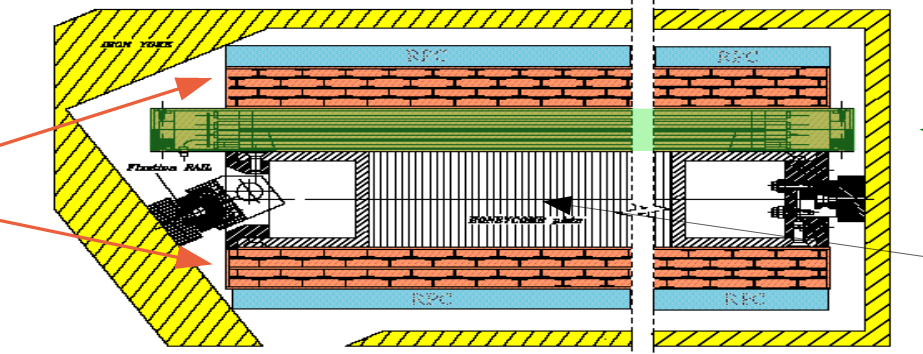
\includegraphics[width=0.45\textwidth]{Chapters/xLHCMS/DTchamber.png}
    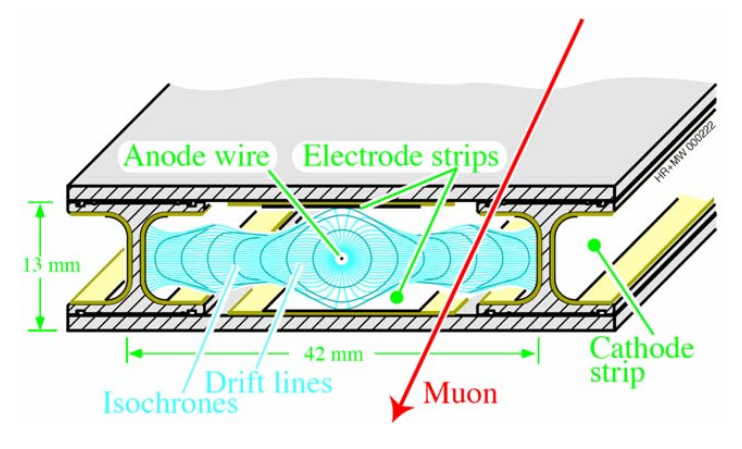
\includegraphics[width=0.45\textwidth]{Chapters/xLHCMS/DTcell.png}
    \caption{Drift Tube chamber and cell design. Left: full DT chamber
    design, including iron yoke (yellow), and RPCs
    (blue), $r-\phi$ Super Layers (in red and pointed by red arrows),
    fixation rail and honeycomb (black), $r-z$ Super Layer
    (green). Each SL contains 4 layers of DT cells. Right: design of a
    single DT cell. High voltage of -1.2, +1.8, +3.6 kV is applied to
    cathode, strips and wires, respectively.}
    \label{fig:DTchamber}
  \end{center}
\end{figure}

The gas mixture inside a drift cell is 85\% argon, 15\% carbon
dioxide. The drift cell contains a 50-$\mu$m-diameter gold plated
anode wire, two 50-$\mu$m-thick aluminium tape acting as electrode on
top and bottom, 23
mm of insulating mylar tape, and a cathode made of 50-$\mu$m-thick
aluminium foil, insulated from the next cell with a 100-$\mu$m-thick
mylar tape layer. The full drift cell design is laid out in
Figure~\ref{fig:DTchamber}, right.


% CSC
In the endcap regions of CMS, the muon rates and background levels are
higher; There, CSC provide a radiation resistant solution, with fine
segmentation and fast response time. The CSCs cover the range
$0.9 < \vert\eta\vert < 2.4$. The endcap wheels being perpendicular to
the beam line, the CSC strips are in the radial plane and provide a
precise measurement in the $r-\phi$ plane.  The anode wires are
perpendicular to the strips, and their readout provides a
pseudorapidity measurement and the coincidence of the muon passing
through with its beam-crossing time. All six CSC layers informations
are used in pattern recognition for non-muon rejection and provide a
helpful anchor point for matching between stations and tracker hits.

The CSCs are multiwire proportional chambers (MWPC), containing 6
anode wire planes interleaved with 7 cathode panels. The schematic CSC
design is shown in Figure~\ref{fig:mwpc} (left). The wires are
aligned in azimuth and used to get the radial coordinate. Strips are
carved into cathode panels aligned at constant $\Delta\phi$ width. The
muon $\phi$ coordinate is then obtained by collection of ionisation
charge on the cathode strips close to where the muon passed. The
repeated measurement of charges collected over the six planes of
strips can be correlated to measure unambiguously the trajectory of
the muon, as is shown in Figure~\ref{fig:mwpc} (right).


\begin{figure}[htb]
  \begin{center}
    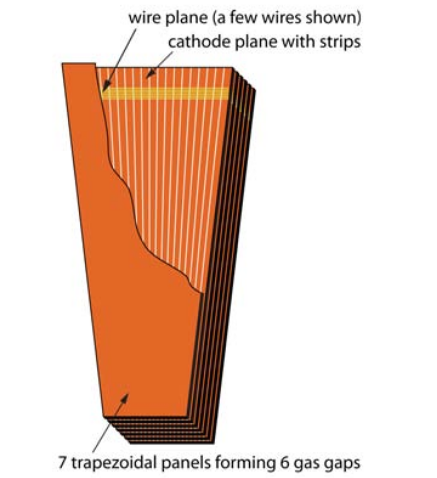
\includegraphics[width=0.4\textwidth]{Chapters/xLHCMS/mwpc.png}
    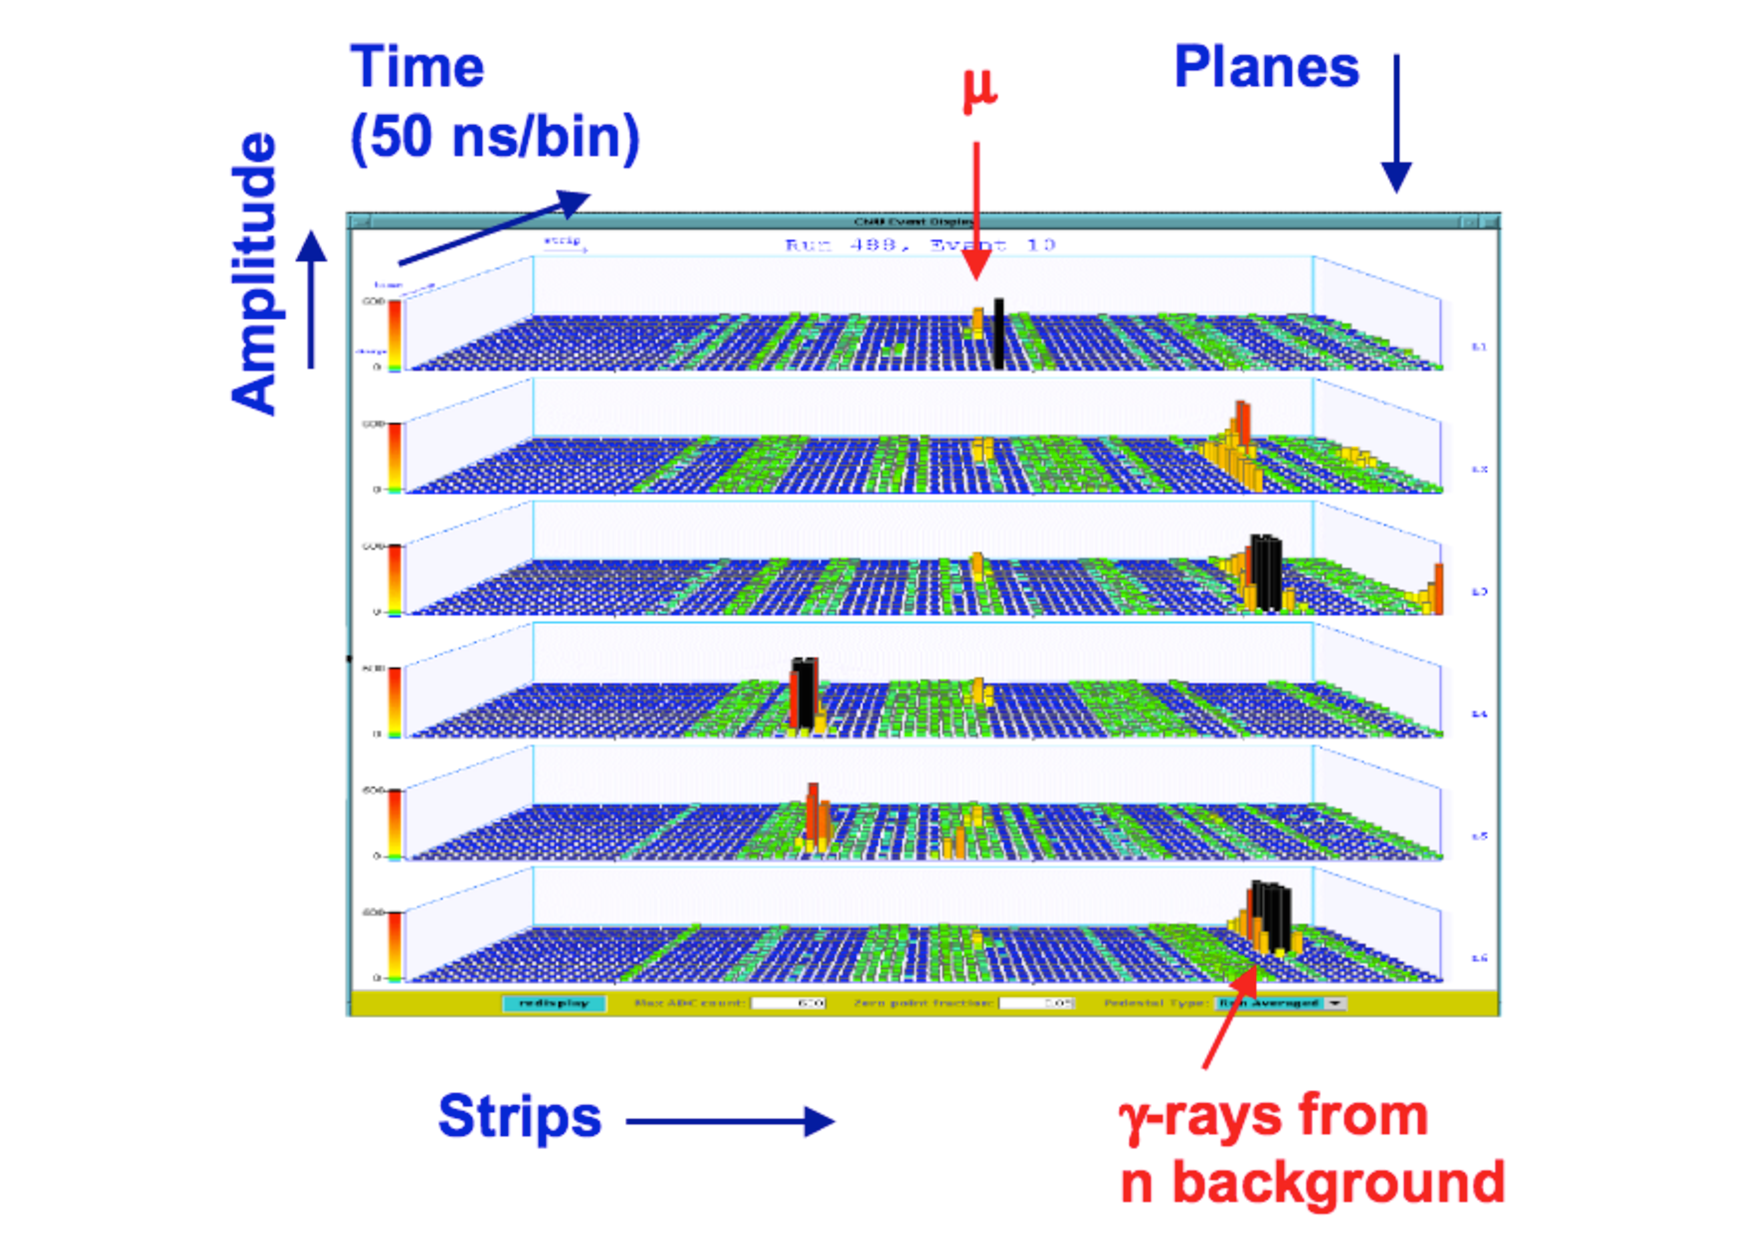
\includegraphics[width=0.5\textwidth]{Chapters/xLHCMS/mwpcmuon.pdf}
    \caption{CSC schematic design, and effect of background and muon
      signals on charge collection. The
    muon track path can be seen passing in the middle of all 6 planes,
    with surrounding spurious spikes identified as background.}
    \label{fig:mwpc}
  \end{center}
\end{figure}

Over the two endcaps, 540 CSC chambers are deployed in 2 times 4 disks
(or stations), covering an active area of 6 000 square meters, and
overlapping in $\phi$ and $\eta$ to reduce dead regions. The CSCs
count 2.5 million wires total. Although the CSC system is very
precise, it is also relatively slow: full charge recollection can take
up to 300~nanoseconds. The data acqusition chain is detailed in~\cite{Chatrchyan:2008aa}.

% RPC



In the initial design of the LHC and CMS, the actual nominal
luminosity and muon rates were not well known. To overcome the
possibility of saturated muon chambers, a third system was added. The
RPCs provide a fast and independent measurement of the muons, with
a sharp momentum threshold, very useful in triggering on the proper
muon-beam-crossing combinations. RPCs are double gap chambers
surrounding the DT or CSC modules, also helpful to resolve ambiguities when
multiple track-hit combinations are formed at the track reconstruction
step.

A RPC is capable of tagging the muon ionisation time faster than 25~ns, making it an efficient first level muon trigger.


At present, there are two layers of (double gap) RPC chambers in the
two inner stations, and one RPC chamber per outer muon station. In the
barrel region, the RPCs thus form 6~coaxial cylinders around the beam
axis. Chambers are approximately 2~meters long and their widths vary
from 1.5~to 2.5~meters. As seen in Figure~\ref{fig:DTchamber}, the
innermost barrel RPCs surround the DT chambers, while for the two
outer stations they are placed before DT chambers.


The double gap structure is detailed here: two strips of bakelite (in
red in Figure~\ref{fig:RPC} left), a
highly resistive plastic material, are placed 2 millimeters away from each
other and operated at high voltage (9 kV). Between the bakelite layers
a gas mixture of tetrafluoroethane, tetraprotonated ethane
(C$_2$H$_2$F$_4$ and C$_2$H$_{10}$) and water vapour is inserted. The
full system operates in avalanche mode (quick appearance of current
flow after a muon passes through). When the muon passes inside the
RPC gaps, copper strips (on top of Figure~\ref{fig:RPC} left) collect
charges within 1 nanosecond. The system described here
represents a single gap: the double gap is obtained by duplicating the
system, improving dramatically the charge collection for minimally
ionising particles such as muons. 


To minimise further the time taken to readout information from RPCs,
the double gaps are lined up two by two in a RPC plane, with a
front-end readout
board running in the middle, along the closest side of the RPC to the
interaction point and perpendicular to the beam line. For example, the
$z$ axis displayed in the schematic design of
Figure~\ref{fig:RPC} (right) shows the beam line direction, and points
toward the beamspot. 


\begin{figure}[htb]
  \begin{center}
    \includegraphics[width=0.4\textwidth]{Chapters/xLHCMS/rpcbarrel.png}
    \includegraphics[width=0.5\textwidth]{Chapters/xLHCMS/rpclayers.jpg}
    \caption{RPC system outline. Left: schematics of a barrel RPC
      chamber, as described in text. Right: exploded view of subparts
      of a RPC, gas is trapped between the two bakelite (red) layers~\cite{RPC}.}
    \label{fig:RPC}
  \end{center}
\end{figure}

Endcap RPC chambers do not differ a lot from the structure outlined
here: placed around or upstream of CSCs, the chambers are also
consisting of double-gap bakelite-and-strip gas chambers. There size
is trapezoidal to fit in the endcap wheel, and the strip run radially.

%\subsection{}

\vspace{0.5em}
\begin{center}
  \fbox{
    \parbox{0.9\textwidth}
    {\textsf {In this Chapter, details of the LHC machine were
        presented. This particle collider of an unprecedented scale is
      equipped with four large experiments. The Thesis presented here
      relies on data from the CMS experiment, whose prime asset is
      the fast and efficient muon subdetector equipment. The CMS
      experiment was originally designed to detect rare events in $pp$
      collisions, but proved efficient in heavy ion environments as
      well. This ability will be covered in Chapter~\ref{chap:xmuons}.
      }}} 
\end{center}


